\chapter{Realisierung}
\label{ref:realisierung}
\subsection{Externe Libraries}
\textbf{ORMLite (Version 4.39)}

Zur Speicherung der Objekte in die SQLite Datenbank des Tablet wird die Java Library ORMLite der Version 4.39 benutzt. In der Zwischenzeit sind neue Releases der Library auf der Webseite \url{http://ormlite.com/releases/} erschienen. Um sich in die Library einzulesen wird auf \url{http://ormlite.com/sqlite_java_android_orm.shtml} verwiesen.
\\
Um eine Änderung an den zu persistierenden Objekten durchzuführen ist es notwendig, die Klasse DatabaseConfigUtil.java im

\lstinline|Package ch.hsr.sa.radiotour.technicalservices.database;|

als normale Java Applikation auszuführen. Dies generiert das \textit{Configuration File}

\lstinline|res/raw/ormlite_config.txt|

welches für eine effizientere Ausführung von \textit{ORMLite} gebraucht wird.

\subsection{Aktuelle Erscheinung}
Die RadioTour App besteht aus einer Activity. Diese Activity wird in zwei Hauptteile eingeteilt. Es sind dies der (1)Header- sowie der (2)Hauptbereich. 

Activity:
\begin{lstlisting}{Name}
package ch.hsr.sa.radiotour.activities;
public class RadioTourActivity extends Activity implements
	Observer, OnClickListene
\end{lstlisting}


View definiert in:
\lstinline|res/layout/base_activity.xml|

\begin{figure}[h!]
\caption{Gesamte Activity}
\centering
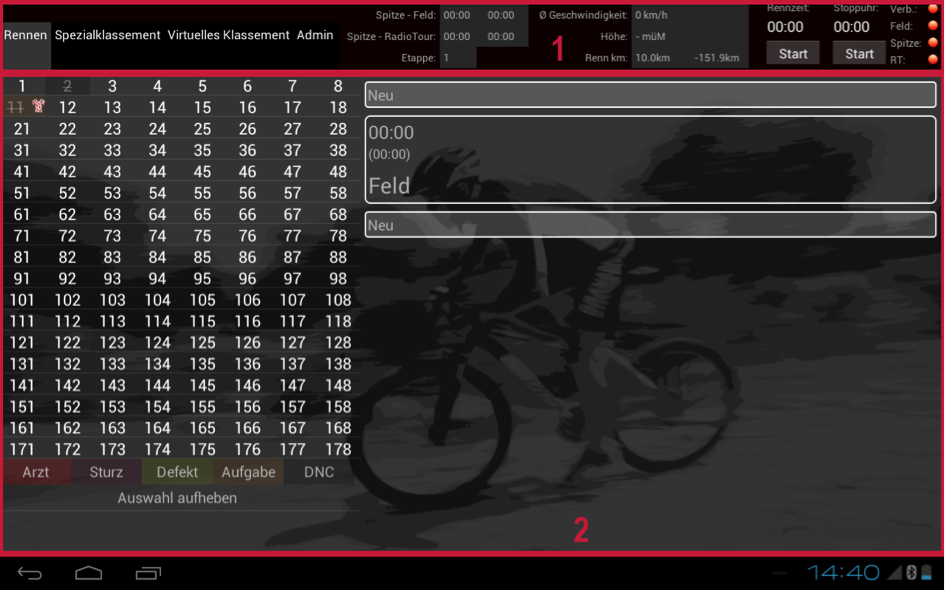
\includegraphics[scale=0.9]{07anhang/images/dev_activity.png}
\end{figure}

\subsection{Headerbereich}

\begin{figure}[h!]
\caption{Header Bereich}
\centering
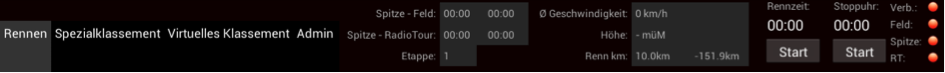
\includegraphics[scale=0.9]{07anhang/images/dev_header.png}
\end{figure}


\begin{lstlisting}{Name}
package ch.hsr.sa.radiotour.fragments;
public class HeaderFragment extends Fragment implements Observer, TimePickerIF
\end{lstlisting}

View definiert in:
\lstinline|res/layout/header_fragment.xml|

\subsection{Hauptbereich}
Der Hauptbereich wird je nach ausgewähltem Tab (im Headerbereich) mit einem anderen Fragment ausgefüllt
RaceFragment.java

\begin{lstlisting}{Name}
package ch.hsr.sa.radiotour.fragments;
public class RaceFragment extends Fragment 
\end{lstlisting}


View definiert in:
\lstinline|res/layout/race_layout.xml|

\begin{figure}[h!]
\caption{RaceFragment}
\centering
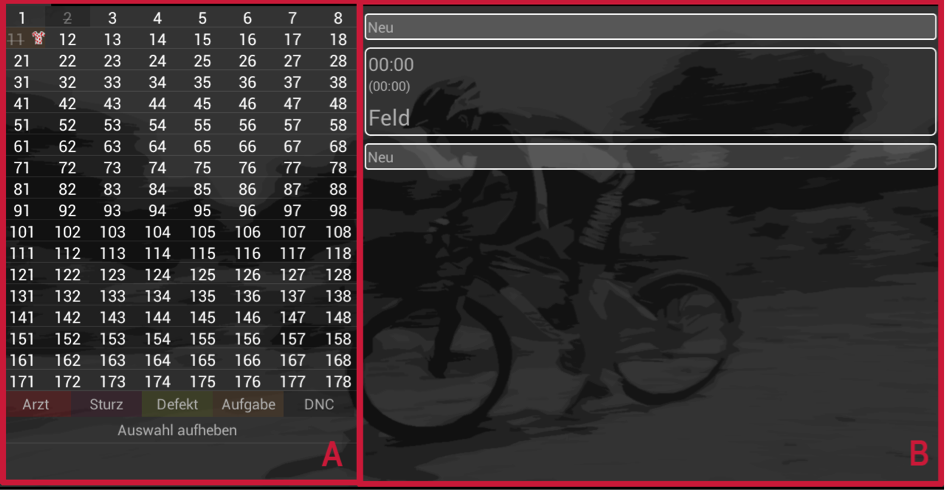
\includegraphics[scale=0.9]{07anhang/images/dev_racefragment.png}
\end{figure}

A RiderPickerFragment
\begin{lstlisting}{Name}
package ch.hsr.sa.radiotour.fragments;

public class RiderPickerFragment extends ListFragment implements OnClickListener
\end{lstlisting}


B RiderGroupFragment
\begin{lstlisting}{Name}
package ch.hsr.sa.radiotour.fragments;

public class RiderPickerFragment extends Fragment
\end{lstlisting}


View definiert in:
\lstinline|res/layout/group_fragment.xml|

\subsection{SpecialRankingFragment}
\begin{lstlisting}{Name}
package ch.hsr.sa.radiotour.fragments;

public class SpecialRankingFragment extends Fragment
\end{lstlisting}

View definiert in:
\lstinline|res/layout/special_ranking_fragment.xml|

\begin{figure}[h!]
\caption{Gesamte Activity}
\centering
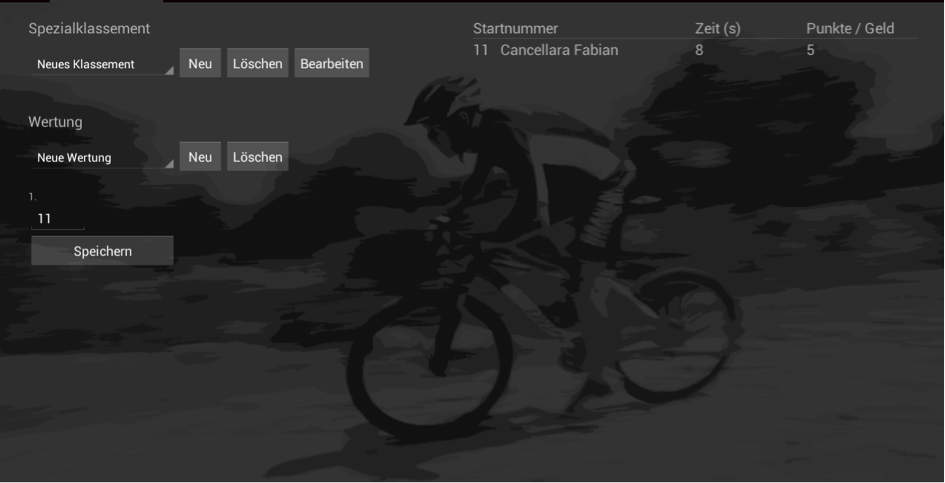
\includegraphics[scale=0.9]{07anhang/images/dev_specialranking.png}
\end{figure}


VirtualRankingFragment
\begin{lstlisting}{Name}
package ch.hsr.sa.radiotour.fragments;

public class VirtualRankingFragment extends ListFragment
\end{lstlisting}


\begin{figure}[h!]
\caption{VirtualRankingFragment}
\centering
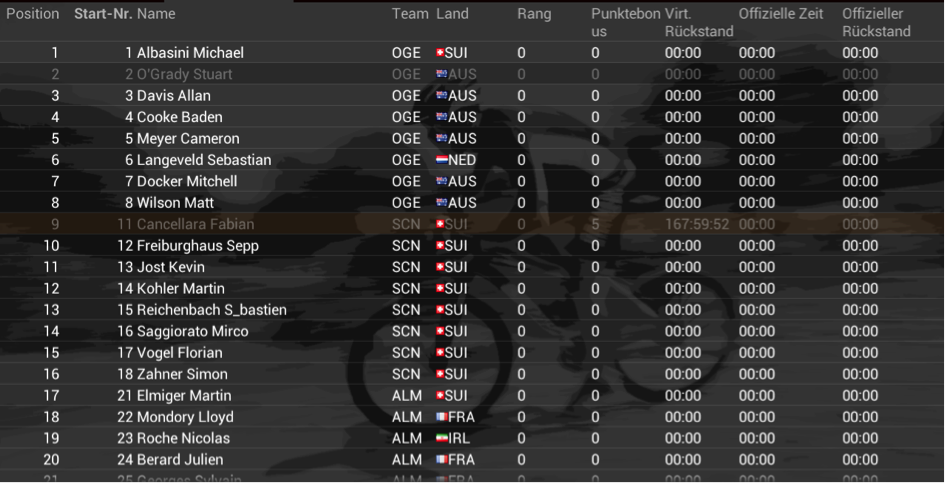
\includegraphics[scale=0.9]{07anhang/images/dev_virtual.png}
\end{figure}

AdminFragment
\begin{lstlisting}{Name}
package ch.hsr.sa.radiotour.fragments;

public class AdminFragment extends Fragment
\end{lstlisting}


View definiert in:
\lstinline|res/layout/admin_fragment.xml|
 
\begin{figure}[h!]
\caption{AdminFragment}
\centering
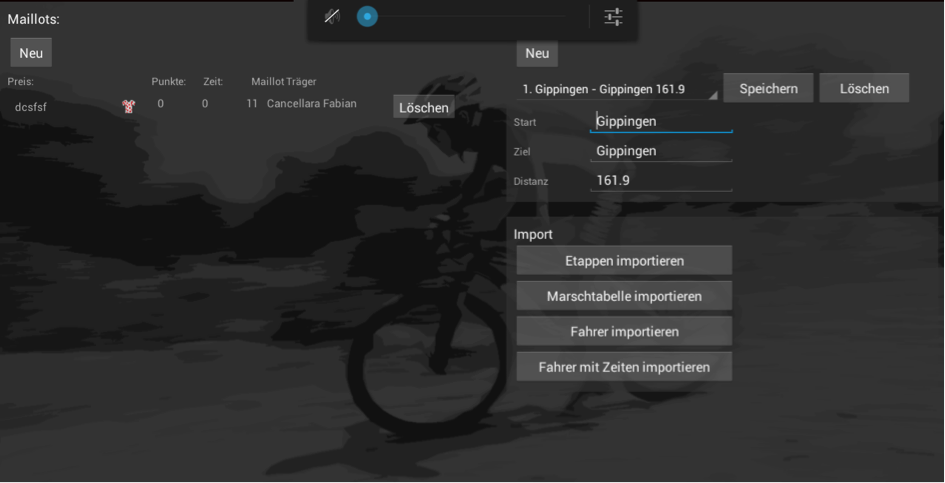
\includegraphics[scale=0.9]{07anhang/images/dev_adminfragment.png}
\end{figure}

\subsection{Offene Tasks}
Die Applikation ist weitgehend einsatzbereit. Folgende weitere Features sind noch offen:
\begin{itemize}
\item JSON
\item Importieren der Fahrerliste sowie der Etappeninformationen ist derzeit als .csv nur via USB möglich
\item Zeitabstände Feld-Spitze
\item Die Zeit- und Punkteboni der Maillots werden noch nicht im virtuellen Klassement verrechnet
\item Bei der Marschtabelle werden die abgefahrenen Stationen ausgegraut jedoch wird nicht auf die aktuelle Position „gescrollt“
\item Beim Wechsel einer Etappe wir die Rennzeit und der Rennkilometer nicht zurückgesetzt
\end{itemize}
